% !TEX root = ../master-thesis.tex

% \textbf{Frequency to position mapping.}
To extract the local intensities $P_{ij}$ from camera images, we need to determine which pixels correspond to which tweezer sites. For this purpose, we define an affine transformation from the drive frequency space $(\omega_{\mathrm{hor}}, \omega_{\mathrm{ver}})$ to image plane coordinates $(x, y)$:
\begin{equation*}
    \vc{r} = H \vc{\omega},
    \hspace{5 mm} \Leftrightarrow \hspace{5 mm} 
    \begin{pmatrix}
        x \\ y
    \end{pmatrix} = \begin{pmatrix}
        h_{11} & h_{12} & h_{13} \\
        h_{21} & h_{22} & h_{23}
    \end{pmatrix} 
    \begin{pmatrix}
        \sub{\omega}{hor} \\
        \sub{\omega}{ver} \\
        1
    \end{pmatrix}.
\end{equation*}
Here, $H$ is a $2 \times 3$ matrix calibrated from a set of measured spot positions. For example, one can measure $\vc{r}_j$ for random frequency vectors $\vc{\omega}_j \in [\omega_{\mathrm{min}},\, \omega_{\mathrm{max}}]$, construct the matrices $\omega_{ij}$ with $i \in \{\mathrm{hor}, \mathrm{ver}\}$ and $r_{ij}$ with $i \in \{x, y\}$, and solve the least-squares problem:
\begin{equation}
    r = H \omega,
    \hspace{0.5cm} \Rightarrow \hspace{0.5cm}
    r \omega^\mathrm{T} = H \omega \omega^\mathrm{T}
    \hspace{0.5cm} \Rightarrow \hspace{0.5cm}
    r \omega^\mathrm{T} \left(\omega \omega^\mathrm{T}\right)^{-1} = H.
    \label{eq:linreg-freq2pos}
\end{equation}
This transformation defines a region of interest around each tweezer, within which we compute the integrated pixel intensity after background subtraction. The resulting values are proportional to the optical powers $P_{ij}$.

% \textbf{Linear reconstruction.}
The mapping from input amplitudes $\vc{a}$ to optical power is approximated by Eq.~\eqref{eq:taylerexp}. In the regime $a_i \in [0.85, 0.95]$, a linear approximation is sufficient\footnote{
    For wider amplitude ranges, higher-order terms can be added to the model. However, this is unnecessary in the present context.
}. We construct the Jacobian matrix $F'_{ji}$ by fitting a linear regression model to a dataset of amplitude–intensity pairs. The resulting crosstalk matrix is shown in Fig.~\ref{fig:control}b. It is approximately diagonal, with comparable diagonal entries and off-diagonal elements typically reaching up to 30\% in magnitude relative to the diagonal, due to power redistribution between neighboring tones. Crosstalk between the horizontal and vertical AODs remains negligible.

The quality of the linear fit for the $4 \times 4$ array is illustrated in Fig.~\ref{fig:control}e. The total intensity (Fig.~\ref{fig:control}d) scales linearly with the average input amplitude, yielding $R^2 > 0.99$. Relative residuals are normally distributed with width $0.3\%$, confirming the applicability of the model in this range.

% \textbf{Power-aware optimization.}
% \grey{In the presence of limited laser power and finite AOM diffraction efficiency, we prefer solutions where all amplitudes remain close to 1. This preference can be incorporated into the optimization objective. In addition to minimizing intensity imbalance, we penalize deviations of the average amplitudes from a target value (e.g., 0.9).}


\begin{figure}
    \centering
    \addletter{140}{a}
    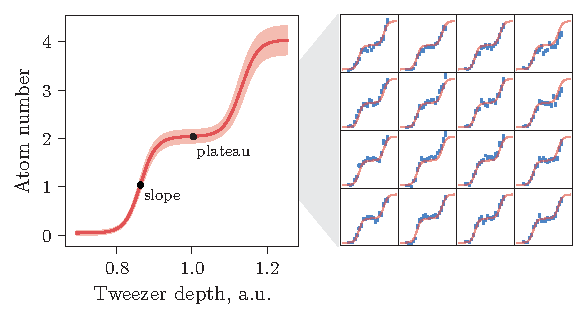
\includegraphics{fig-ai/step-plot-joined.pdf}
    \phantom{42}
    \addletter{140}{b}
    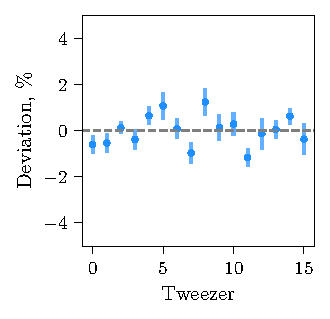
\includegraphics{fig-py/step-plot-balance.pdf} % 0.6 +- 0.2
    % 
    % 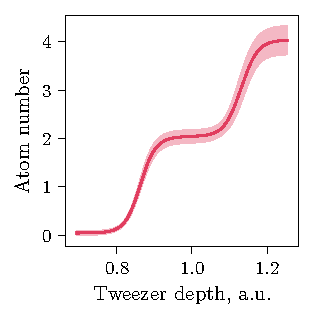
\includegraphics{fig-py/step-plot.pdf}
    % 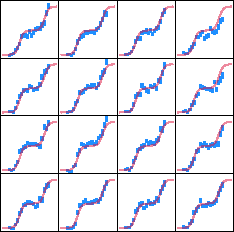
\includegraphics{fig-py/step-plot-inset.pdf}
    \caption[Step plot]{
        \textbf{Step plot.}
        (a) 
        Atom number as a function of tweezer depth during the spilling sequence. 
        % Plateaus correspond to quantized energy levels of the 1D harmonic oscillator. 
        Step plots for each tweezer in the $4 \times 4$ array are shown on the right. The average fit is shown as a solid red line, with standard deviation across sites indicated by the shaded area. 
        (b) Relative deviation of the fitted sigmoid centers for each tweezer after SVF balancing. The standard deviation is $0.7(2)\%$, which is well within the plateau width ($\pm 5\,\%$), ensuring sufficient uniformity for array-wide spilling.
        % All measurements were performed in this work using atom-based measurements and SVF-balanced tweezer depths.
    }
    \label{fig:stepplot}
\end{figure}